%\documentclass[11]{beamer}
\documentclass[aspectratio=169]{beamer}

% Pacotes
\usepackage[T1]{fontenc} 
\usepackage[utf8]{inputenc} % Ambos corrigem os problemas de encoding
\usepackage{lmodern}  % Font que tenta corrigir as alterações dos pacotes anteriores
\usepackage[portuguese]{babel} % Modificar certos nomes para português
\usepackage{ragged2e} % Justificar texto

% Definições do tema
\usetheme{copenhagen}
\usecolortheme{default}

% Alterações ao template
\setbeamertemplate{navigation symbols}{} % Remove os símbolos de navegação
\setbeamertemplate{headline}{} % Remove o cabeçalho
\setbeamertemplate{footline}[frame number] % Adiciona o número do slide ao canto inferior direito

% Informação da capa:
\title{Ferramenta para Geração de Horários de Cursos com Restrições}
\subtitle{Apresentação do Relatório de Desenvolvimento do Trabalho}

\author[Ricardo Ramos]{Ricardo Alexandre Alves Ramos}

\institute[ISEL]{Instituto Superior de Engenharia de Lisboa}

\date{\today}

\institute{
    Instituto Superior de Engenharia de Lisboa \\ 
    Departamento de Engenharia Eletrónica e de Telecomunicações e Computadores \\ 
    Mestrado em Engenharia Informática e de Computadores
}

\begin{document}
    %----------------------------------------------------------------------------------------
    %    PRESENTATION SLIDES
    %----------------------------------------------------------------------------------------

    % Slide de título
    \begin{frame}[t,plain]
        \begin{center}
            \begin{beamercolorbox}[rounded=true, shadow=true, sep=10pt, center, wd=\linewidth]{title}
                \color{white} \usebeamerfont{title} \textbf{\inserttitle} \\
                \usebeamerfont{subtitle} \insertsubtitle
            \end{beamercolorbox}
            
            \vspace{1em}
            {\usebeamerfont{author} \insertauthor}

            \vspace{1em}
            {\footnotesize
            Orientadores: Prof. Doutor Nuno Miguel da Costa de Sousa Leite \\
            \vspace{-1mm}\hspace{-.5cm}Prof. Doutor Artur Jorge Ferreira}
            
            \vspace{1em}
            {\usebeamerfont{institute} \insertinstitute}
            
            \vspace{2em}
            {\usebeamerfont{date} \insertdate}

            \vspace{-1.5em}\hspace{7.5cm}
            
\includegraphics[width=2.5cm]{img/logoisel.png}
        \end{center}
    \end{frame}

    \begin{frame}{Índice}
        \tableofcontents
    \end{frame}

    %------------------------------------------------
    \section{Introdução}
    %------------------------------------------------

    \begin{frame}{Problemas de Agendamento (1/2)}
        \justifying

        Os problemas de agendamento são da classe de otimização combinatória. Estes problemas existem em várias áreas como:
        \begin{itemize}
            \item Ensino
            \item Medicina
            \item Transporte
            \item Logística
        \end{itemize}
        \vfill

        Na área de ensino, os problemas de agendamento podem ser abordados por meio de duas formulações:
        \begin{itemize}
            \item Agendamento de Disciplinas Baseado no Currículo (CB-CTT)
            \item Agendamento de Disciplinas Após Inscrição (PE-CTT)
        \end{itemize}
    \end{frame}

    \begin{frame}{Problemas de Agendamento (2/2)}
        \justifying

        Os problemas de agendamento escolar podem ainda ser divididos em três categorias:
        \begin{itemize}
            \item Agendamento Escolar (\textit{School Timetabling})
            \item Agendamento de Cursos Universitários (\textit{Course Timetabling})
            \item Agendamento de Exames (\textit{Examination Timetabling})
        \end{itemize}
        
        \vfill

        Este projeto terá como objetivo a criação de uma ferramenta com interface gráfica, que permita a criação de horários, com um foco na categoria de Agendamento de Cursos Universitários, com a formulação Agendamento de Disciplinas Baseado no Currículo.
    \end{frame}

    %------------------------------------------------
    \section{Estado da Arte}
    %------------------------------------------------

    \subsection{Algoritmos tipicamente utilizados}

    \begin{frame}{Algoritmos tipicamente utilizados}
        \justifying

        Algoritmos utilizados:
        \begin{itemize}
            \item Coloração de Grafos (\textit{Graph Coloring})
            \item Coloração de Arestas (\textit{Edge Coloring})
            \item Programação Inteira (\textit{Integer Programming})
            \item Procura Tabu (\textit{Tabu Search})
            \item Têmpera Simulada (\textit{Simulated Annealing})
        \end{itemize}

        \vfill

        Nos últimos anos, a utilização de algoritmos híbridos tem aumentado, combinando diferentes técnicas para melhorar o seu desempenho e a sua eficiência na resolução destes problemas.
    \end{frame}

    \subsection{Empresa \textit{Bullet Solutions}}

    \begin{frame}{Empresa \textit{Bullet Solutions} (1/2)}
        \justifying

        A empresa \textit{Bullet Solutions} é uma empresa tecnológica especializada no desenvolvimento de soluções para otimização de recursos e gestão de horários.

        \vfill

        A criação dos horários começa com uma solução inicial, gerada através de uma heurística sequencial.

        \vfill

        A técnica de otimização é uma heurística criada e adaptada ao problema, utilizando conceitos e princípios de outras meta-heurísticas, sendo uma delas o \textit{Tabu Search}.

        \vfill

        O projeto será desenvolvido com o objetivo de oferecer uma alternativa competitiva à aplicação disponibilizada pela \textit{Bullet Solutions}, que é atualmente utilizada no ISEL.
    \end{frame}

    \begin{frame}{Empresa \textit{Bullet Solutions} (2/2)}
        \justifying
        Solução disponibilizada pela \textit{Bullet Solutions}:
        \begin{center}
            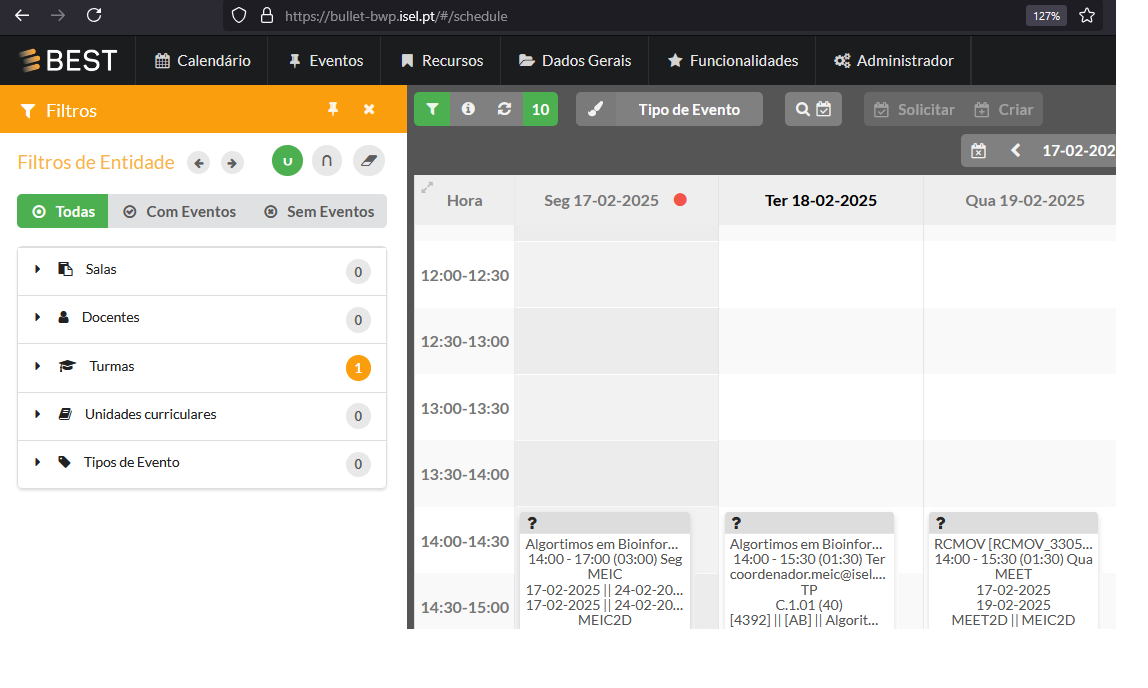
\includegraphics[width=10cm]{img/exemplo-bullet-solutions-software.png}
        \end{center}
    \end{frame}
    
    \subsection{ITC 2019}

    \begin{frame}{ITC 2019}
        \justifying
        A ITC 2019 teve um foco na elaboração de horários em contextos educacionais, como a criação de horários para escolas e universidades.

        \vfill
        
        A competição disponibiliza o padrão a ser utilizado e alguns dados para efeitos de comparação de resultados.

        \vfill
        
        O padrão disponibilizado permite o armazenamento dos seguintes dados:
        \begin{itemize}
            \item Cursos
            \item Alunos
            \item Disciplinas
            \item Restrições
        \end{itemize}

        \vfill

        Para permitir a utilização do padrão no projeto, foi feita uma extensão para acrescentar os dados dos professores.
    \end{frame}

    %------------------------------------------------
    \section{Trabalho Realizado}
    %------------------------------------------------

    \subsection{Diagrama de blocos}

    \begin{frame}{Diagrama de blocos}
        %Diagrama de blocos:
        \begin{center}
            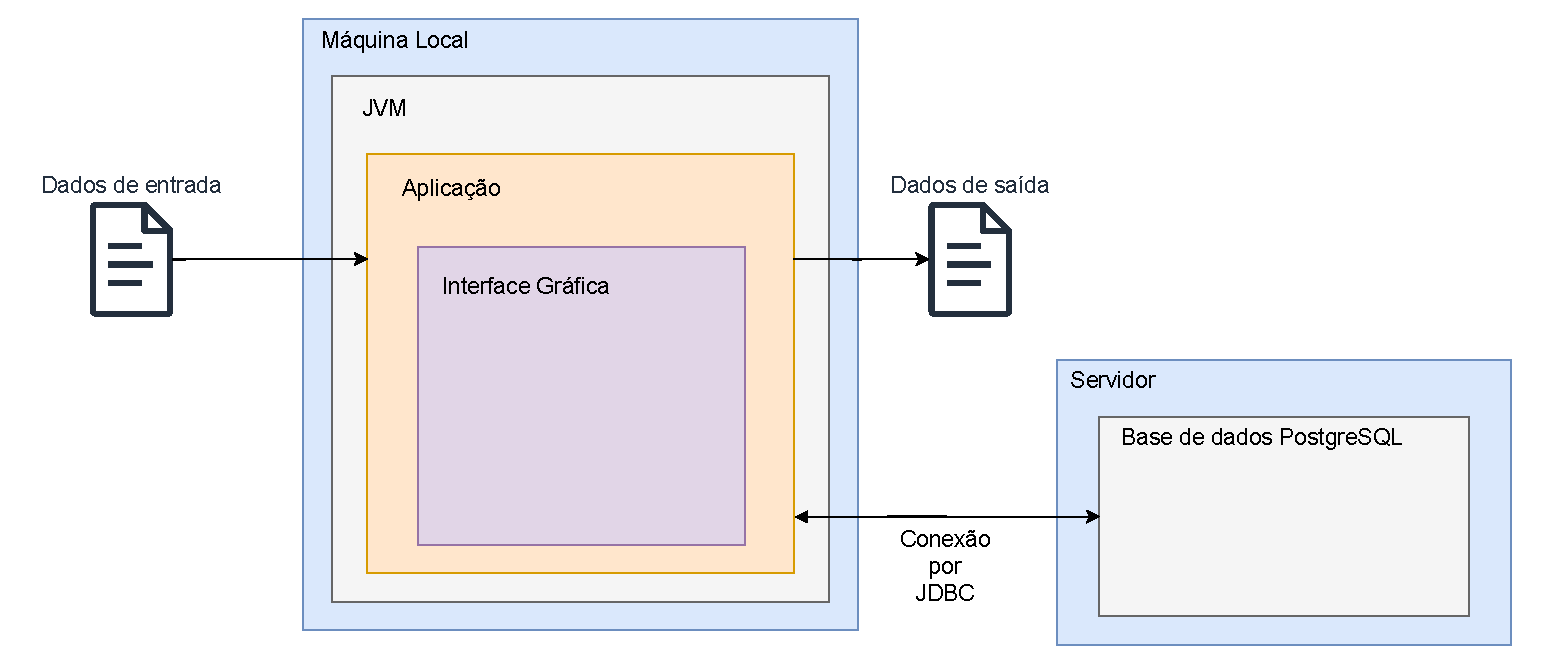
\includegraphics[width=\linewidth]{img/diagrama-blocos-slides.pdf}
        \end{center}
    \end{frame}

    \subsection{Dados de entrada e saída}

    \begin{frame}{Dados de entrada e saída}
        \justifying

        Tipo dos ficheiros de entrada:
        \begin{itemize}
            \item XML seguindo o padrão proposto
        \end{itemize}

        \vfill

        Tipos dos ficheiros de saída:
        \begin{itemize}
            \item CSV e XML para todos os dados armazenados
            \item PNG e PDF apenas para os horários gerados
        \end{itemize}
    \end{frame}

    \subsection{Vantagens das tecnologias a utilizar}

    \begin{frame}{Vantagens das tecnologias a utilizar (1/2)}
        \justifying
        Vantagens da linguagem Java:
        \begin{itemize}
            \item O programa pode ser executado em qualquer sistema operativo
            \item Vasta coleção de bibliotecas
            \item Rápido e eficiente
        \end{itemize} 

        \vfill

        A utilização do JDBC tem as seguintes vantagens:
        \begin{itemize}
            \item Simplicidade de implementação
            \item Controlo total nas transações
        \end{itemize}
    \end{frame}

    \begin{frame}{Vantagens das tecnologias a utilizar (2/2)}
        \justifying
        As vantagens da utilização do PostgreSQL são as seguintes:
        \begin{itemize}
            \item Eficiente e escalável para grandes volumes de dados
            \item Suporta replicação
            \item Suporta transações concorrentes
        \end{itemize}
    \end{frame}

    \subsection{Tarefas realizadas}

    \begin{frame}{Tarefas realizadas}
        \justifying

        %Tarefas realizadas:
        \begin{itemize}
            \item Definição do contexto e objetivos do projeto
            \item Análise das técnicas propostas na literatura
            \item Definição do diagrama de blocos
            \item Definição dos requisitos funcionais e não funcionais
            \item Análise detalhada do padrão proposto na ITC 2019
            \item Extensão do padrão
            \item Definição dos casos de utilização
            \item Definição das restrições dos horários
        \end{itemize}

    \end{frame}

    %------------------------------------------------
    \section{Trabalho Futuro}
    %------------------------------------------------

    \subsection{Diagrama de Gantt}

    \begin{frame}{Diagrama de Gantt}
        \justifying

        \begin{figure}
            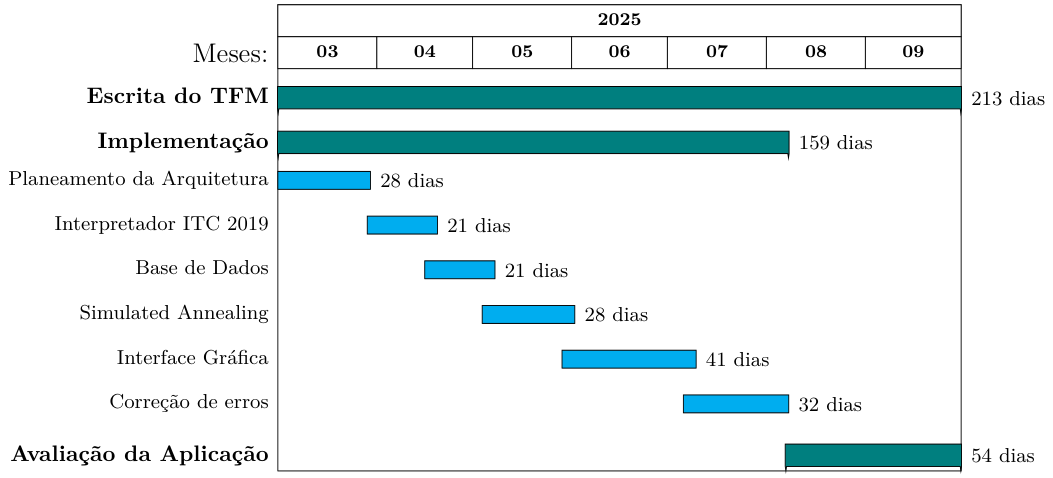
\includegraphics[width=.85\linewidth]{img/Diagrama-Gantt.png}
        \end{figure}

        \vfill

        Maiores riscos:
        \begin{itemize}
            \item Criação de uma interface gráfica eficiente e intuitiva
            \item Implementação do \textit{Simulated Annealing} e lógica de criação de horários
        \end{itemize}

        \vfill
    \end{frame}

    \subsection{Tarefas Principais}

    \begin{frame}{Tarefas Principais (1/2)}
        \justifying

        Implementações previstas:
        \begin{enumerate}
            \item Sistema para importação de dados XML que sigam o padrão proposto
            \item Importação manual dos dados
            \item Apresentação de erros ao utilizador em caso de falha no sistema
            \item Apresentação dos conflitos no caso de impossibilidade de criação de horários
            \item Interface gráfica intuitiva e eficiente
            
            \newcounter{tarefasPrincipais}
            \setcounter{tarefasPrincipais}{\value{enumi}}
        \end{enumerate}
    \end{frame}

    \begin{frame}{Tarefas Principais (2/2)}
        \justifying
        Implementações previstas:
        \begin{enumerate}
            \setcounter{enumi}{\value{tarefasPrincipais}}

            \item Permitir ajustes manuais aos horários gerados
            \item Algoritmo SA e otimização dos seus parâmetros 
            \item Base de dados para a persistência dos dados
            \item Apresentação de retorno visual durante o processo de geração de horários
        \end{enumerate} %TODO: Confirmar a alteração de feedback para retorno
    \end{frame}

    \subsection{Tarefas Secundárias}

    \begin{frame}{Tarefas Secundárias}
        \justifying

        Implementações previstas caso as tarefas principais estejam concluidas:
        \begin{enumerate}
            \item Definição de manchas de disponibilidade através da interface gráfica
            \item Definição de períodos para aulas partilhadas através da interface gráfica
            \item Criação de registos detalhados do funcionamento do sistema
            \item Congelamento de salas e/ou professores no momento de geração de horários
        \end{enumerate}
    \end{frame}

    %----------------------------------------------------------------------------------------

\end{document}